\documentclass[
   ngerman
  ,a4paper
  ,12pt
  ,pdftex
  ,disable
]{report}

\usepackage[utf8]{inputenc}        
\usepackage{bericht}


\csname endofdump\endcsname

\newcommand{\Kursbezeichnung}{TINF23B3}


\newcommand{\Titel}{Dokumentation PIC Simulator}
\newcommand{\AbgabeDatum}{12. Mai 2025}

\includeonly{
  abk
 ,kapitel1‚
 ,kapitel2
 ,kapitel3
 ,changelog
}

\begin{document}

\pagenumbering{roman}

\begin{titlepage}
\begin{center}
\vspace*{-2cm}
\hfill
\includegraphics[width=4cm]{dhbw-logo}\\[2cm]
{\Huge \Titel}\\[1.5cm] 

\begin{tabular}{l@{\hspace{2cm}}l}
Abgabedatum			         & \AbgabeDatum		\\  
Kurs			         & \Kursbezeichnung		\\
Autoren	 & Luca Müller		\\
	        & Leander Gantert		\\
\end{tabular}
\end{center}
\end{titlepage}


\begin{abstract}
Dieses \LaTeX-Dokument kann als Vorlage für einen Praxis- oder Projektbericht, eine Studien- oder
Bachelorarbeit dienen.

\end{abstract}

\newpage
\tableofcontents           
\listoffigures             
%\listoftables              
\lstlistoflistings         


%%%%%%%%%%%%%%%%%%%%%%%%%%%%%%%%%%%%%%%%%%%%%%%%%%%%%%%%%%%%%%%%%%%%%%%%%%%%%%
%% Descr:       Vorlage für Berichte der DHBW-Karlsruhe, Datei mit Abkürzungen
%% Author:      Prof. Dr. Jürgen Vollmer, vollmer@dhbw-karlsruhe.de
%% $Id: abk.tex,v 1.4 2017/10/06 14:02:03 vollmer Exp $
%% -*- coding: utf-8 -*-
%%%%%%%%%%%%%%%%%%%%%%%%%%%%%%%%%%%%%%%%%%%%%%%%%%%%%%%%%%%%%%%%%%%%%%%%%%%%%%%

\chapter*{Abkürzungsverzeichnis}                   % chapter*{..} -->   keine Nummer, kein "Kapitel"
						         % Nicht ins Inhaltsverzeichnis
% \addcontentsline{toc}{chapter}{Akürzungsverzeichnis}   % Damit das doch ins Inhaltsverzeichnis kommt

% Hier werden die Abkürzungen definiert
\begin{acronym}[DHBW]
  % \acro{Name}{Darstellung der Abkürzung}{Langform der Abkürzung}
 \acro{Abk}[Abk.]{Abkürzung}

 % Folgendes benutzen, wenn der Plural einer Abk. benöigt wird
 % \newacroplural{Name}{Darstellung der Abkürzung}{Langform der Abkürzung}
 \newacroplural{Abk}[Abk-en]{Abkürzungen}

 \acro{H2O}[\ensuremath{H_2O}]{Di-Hydrogen-Monoxid}

 % Wenn neicht benutzt, erscheint diese Abk. nicht in der Liste
 \acro{NUA}{Not Used Acronym}
\end{acronym}
              

\pagenumbering{arabic}


\chapter{Einleitung}

\section{Über dieses Dokument}
Dieses Dokument beschreibt einen PIC Simulator, seine Funktionen sowie die Implementierung. Die Dokumentation richtet sich an Benutzer und Entwickler, die den Simulator verstehen möchten.

\section{Projektziele}
Der PIC Simulator wurde entwickelt, um auch in Abwesenheit von physischer Hardware Programme ausführen zu können. Die Hauptfunktionen umfassen:

\begin{itemize}
    \item Simulation von PIC-Mikrocontroller-Programmen
    \item Visualisierung des Programmablaufs
    \item Debugging-Funktionalitäten
\end{itemize}

% Grundlagen
\chapter{Grundlagen}

\section{Grundsätzliche Arbeitsweise eines Simulators}

Ein Simulator ist eine Software, welche das Verhalten eines realen Systems nachbildet. Im Fall eines Mikrocontrollers wie dem PIC wird die Hardwarearchitektur – bestehend aus Central Processing Unit (CPU), Speicher, Registern und Peripheriekomponenten – virtuell nachgebildet, um Programme auszuführen, als würden sie auf der physischen Hardware laufen. Die grundsätzliche Arbeitsweise eines solchen Simulators umfasst typischerweise die folgenden, eng miteinander verzahnten Schritte:

\begin{itemize}
    \item \textbf{Laden des Programms}: Der erste Schritt besteht darin, das zu testende Programm in den simulierten Speicher des Mikrocontrollers zu laden. Dieses Programm liegt in Form einer .LST-Datei vor, die sowohl den Maschinencode als auch die ursprünglichen Assemblerinstruktionen enthält.
    \item \textbf{Dekodieren der Instruktionen}: Nachdem das Programm geladen ist, beginnt der Simulator mit der Ausführung. Dazu liest die simulierte CPU die erste Instruktion aus dem Programmspeicher, auf die der Programmzähler (Program Counter, PC) zeigt. Jede dieser Instruktionen ist ein HEX Code, der vom Simulator dekodiert werden muss. Das Dekodieren bedeutet, den HEX Code zu analysieren, um festzustellen, welcher Befehl ausgeführt werden soll und welche Operanden dafür benötigt werden.
    \item \textbf{Ausführen der Instruktionen}: Nach der Dekodierung führt die simulierte CPU die entsprechende Operation aus. Dies beinhaltet die Manipulation von Daten in den simulierten Registern, das Lesen oder Schreiben von Werten im simulierten Speicher und die Aktualisierung von Statusregistern (Flags), wie z.B. dem Zero-Flag, Carry-Flag oder Overflow-Flag, basierend auf dem Ergebnis der Operation. Nach der Ausführung einer Instruktion wird der Programmzähler in der Regel inkrementiert, um auf die nächste Instruktion zu zeigen, es sei denn, es wurde ein Sprung- oder Verzweigungsbefehl ausgeführt.
    \item \textbf{Interaktion mit Peripherie}: Moderne Mikrocontroller verfügen über eine Vielzahl von integrierten Peripheriegeräten wie Timer/Counter, Interrupt-Controller und digitale Ein-/Ausgabe-Ports (I/O-Ports). Wenn das Programm mit diesen Peripheriegeräten interagiert (z.B. einen Timer startet, einen Wert von einem I/O-Port liest oder einen Interrupt auslöst), muss der Simulator dieses Verhalten ebenfalls nachbilden. Dies kann bedeuten, interne Zustände der simulierten Peripherie zu ändern, simulierte Zeitabläufe zu verwalten oder externe Ereignisse (z.B. ein simuliertes Signal an einem I/O-Pin) zu verarbeiten.
    \item \textbf{Visualisierung und Debugging-Unterstützung}: Ein wesentlicher Aspekt vieler Simulatoren ist die Fähigkeit, den internen Zustand des simulierten Systems dem Benutzer darzustellen. Dies umfasst die Anzeige der aktuellen Werte von CPU-Registern, Speicherinhalten, dem Zustand von Peripheriegeräten und des Stacks.
\end{itemize}

\section{Vor- und Nachteile einer Simulation}

Simulationen bieten zahlreiche Vorteile für den Entwicklungsprozess von Embedded Systems, bringen jedoch auch spezifische Einschränkungen mit sich, die berücksichtigt werden müssen.

\subsection*{Vorteile}
\begin{itemize}
    \item \textbf{Kosteneffizienz}: Einer der größten Vorteile ist die erhebliche Reduktion der Kosten. Es entfallen Ausgaben für die Anschaffung teurer Entwicklungsboards, spezifischer Messgeräte oder Prototypen-Hardware. Auch Kosten für Reparatur oder Ersatz bei Beschädigung durch fehlerhafte Programme oder Experimente entfallen. Dies ermöglicht insbesondere kleineren Teams oder Einzelentwicklern den Zugang zu Entwicklungswerkzeugen.
    \item \textbf{Flexibilität und schnelle Iteration}: Änderungen am Programmcode oder an der simulierten Hardwarekonfiguration, wie beispielsweise die Taktfrequenz oder der angeschlossene Peripherieumfang, können softwareseitig schnell und ohne physischen Umbau vorgenommen werden. Dies beschleunigt den Entwicklungszyklus erheblich, da verschiedene Szenarien und Konfigurationen in kurzer Zeit getestet werden können.
    \item \textbf{Umfassende Debugging-Möglichkeiten}: Simulatoren bieten oft weitreichendere Einblicke in das Systemverhalten als dies mit physischer Hardware möglich wäre. Entwickler können den Programmablauf schrittweise verfolgen (Single-Stepping), Haltepunkte (Breakpoints) an beliebigen Stellen im Code setzen oder den Inhalt von Registern und Speicherbereichen in Echtzeit inspizieren und modifizieren. Auch komplexe Zustände und Zeitabläufe lassen sich detailliert analysieren, was die Fehlersuche und -behebung (Debugging) signifikant erleichtert.
    \item \textbf{Sicherheit und Risikominimierung}: Kritische oder potenziell destruktive Programmzustände können in einer simulierten Umgebung gefahrlos getestet werden. Es besteht kein Risiko, reale Hardware durch fehlerhaften Code, falsche Spannungen oder Kurzschlüsse zu beschädigen. Dies ist besonders wertvoll beim Testen von Grenzfällen oder Fehlerbehandlungsroutinen.
    \item \textbf{Frühzeitige Softwareentwicklung}: Die Softwareentwicklung kann parallel zur oder sogar vor der Fertigstellung der physischen Hardware beginnen. Dies verkürzt die Gesamtentwicklungszeit (Time-to-Market) und ermöglicht eine frühere Validierung von Softwarekonzepten.
    \item \textbf{Automatisierte Tests}: Simulatoren lassen sich gut in automatisierte Testumgebungen integrieren. Testskripte können eine Vielzahl von Szenarien durchlaufen lassen und die Ergebnisse protokollieren, was die Qualitätssicherung verbessert und Regressionstests vereinfacht.
\end{itemize}

\subsection*{Nachteile}
\begin{itemize}
    \item \textbf{Eingeschränkte Genauigkeit und Realitätsnähe}: Eine Simulation ist immer eine Abstraktion der Realität. Insbesondere timing-kritisches Verhalten, analoge Komponenten oder sehr spezifische Hardwareeigenschaften (z.B. exakte Interrupt-Latenzzeiten, Stromverbrauch) können oft nur angenähert oder gar nicht simuliert werden. 
    \item \textbf{Abweichungen zur realen Hardware}: Trotz sorgfältiger Modellierung können immer subtile Unterschiede zwischen dem Verhalten des Simulators und der realen Hardware bestehen. Dies kann an unvollständiger Dokumentation der Hardware, Vereinfachungen im Simulationsmodell oder Fehlern im Simulator selbst liegen. 
    \item \textbf{Entwicklungs- und Wartungsaufwand für den Simulator}: Die Erstellung und Pflege eines genauen und umfassenden Simulators ist selbst ein komplexes Softwareprojekt, das Ressourcen bindet. Insbesondere bei neuen oder sehr speziellen Mikrocontrollern ist möglicherweise kein passender Simulator verfügbar oder muss erst entwickelt werden.
\end{itemize}
 
% Benuteroberfläche
\chapter{Benutzeroberfläche}

Die Benutzeroberfläche des PIC Simulators ist so gestaltet, dass sie eine intuitive und effiziente Nutzung ermöglicht. Im Folgenden werden die wichtigsten Elemente der Benutzeroberfläche und deren Handhabung detailliert beschrieben:

\section{Hauptfenster}
Das Hauptfenster des Simulators ist in mehrere Bereiche unterteilt, die jeweils spezifische Informationen und Funktionen bereitstellen:
\begin{itemize}
    \item \textbf{Code-Editor}: Der integrierte Code-Editor ermöglicht das Laden von Assemblerdateien. Breakpoints können durch einfaches Anklicken der Checkbox am Zeilenanfang gesetzt werden, um den Programmablauf gezielt zu analysieren.
    \item \textbf{Steuerelemente}: Buttons wie \texttt{Go} und \texttt{Reset} steuern die Programmausführung. Diese Steuerelemente sind übersichtlich angeordnet und leicht zugänglich.
    \item \textbf{Register- und Speicheranzeige}: Diese Bereiche zeigen den aktuellen Zustand der Register, Flags und des Speichers in Echtzeit an. Änderungen werden sofort visualisiert, um den Programmablauf nachvollziehbar zu machen und das Debugging zu erleichtern.
    \item \textbf{I/O-Visualisierung}: Die I/O-Pins des Mikrocontrollers werden interaktiv dargestellt. Benutzer können die Zustände der Pins durch Anklicken ändern, um verschiedene Szenarien zu simulieren. Ebenfalls wird angezeigt, ob ein Pin als Eingang oder Ausgang konfiguriert ist.
    \item \textbf{Peripheriegeräte}: Eine Übersicht der simulierten Peripheriegeräte, wie Timer und Interrupts, wird bereitgestellt. Diese Bereiche ermöglichen eine einfache Konfiguration und Überwachung der Peripheriefunktionen.
    \item \textbf{Statusbereich}: Der Statusbereich zeigt wichtige Informationen wie den aktuellen Program Counter (PC), den Stackpointer und die Ausführungszeit an.
\end{itemize}

\section{Menüleiste}
Die Menüleiste bietet Zugriff auf grundlegende Funktionen des Simulators:
\begin{itemize}
    \item \textbf{Datei}: Optionen zum Laden von Quelldateien.
    \item \textbf{Hilfe}: Zugriff auf die Dokumentation.
\end{itemize}

\section{Debugging-Tools}
Die Benutzeroberfläche enthält leistungsstarke Debugging-Tools, die die Fehlersuche erleichtern:
\begin{itemize}
    \item \textbf{Breakpoints}: Benutzer können Breakpoints setzen, um die Programmausführung an bestimmten Stellen zu pausieren und schrittweise fortzusetzen.
    \item \textbf{Speicherüberwachung}: Der Speicherinhalt kann in Echtzeit überwacht und bei Bedarf manuell geändert werden.
    \item \textbf{Registeranzeige}: Alle Register des Mikrocontrollers werden angezeigt, einschließlich ihrer aktuellen Werte. Die Register können ebenfalls manuell bearbeitet werden.
    \item \textbf{Statusflags}: Die Statusflags (z. B. Carry, Zero) werden in Echtzeit aktualisiert und angezeigt, um den aktuellen Zustand des Mikrocontrollers zu verdeutlichen.
\end{itemize}

\section{Visualisierung und Interaktivität}
Die Benutzeroberfläche bietet eine visuelle Darstellung des Mikrocontrollers und seiner Peripherie:
\begin{itemize}
    \item \textbf{Simulation von Peripheriegeräten}: Timer, Interrupts und andere Peripheriegeräte können simuliert und überwacht werden.
    \item \textbf{Echtzeit-Updates}: Änderungen im Programm oder in der Hardwarekonfiguration werden sofort in der Benutzeroberfläche reflektiert.
    \item \textbf{Interaktive Elemente}: Benutzer können direkt mit der Simulation interagieren, z. B. durch das Ändern von I/O-Pin-Zuständen.
    \item \textbf{Konfiguration}: Benutzer können die Taktfrequenz des Simulators anpassen.
\end{itemize}

\section{Zusammenfassung}
Die Benutzeroberfläche des PIC Simulators kombiniert Funktionalität und Benutzerfreundlichkeit. Sie bietet alle notwendigen Werkzeuge, um Programme effizient zu testen und zu debuggen. Durch die klare Struktur und die interaktiven Elemente wird die Arbeit mit dem Simulator erheblich erleichtert.






% Technische Details
\chapter{Technische Details und Funktionsweise}

\section{Warum Python gewählt wurde}
Zur Umsetzung des Projekts wurde Python als Programmiersprache gewählt, da es mehrere Vorteile bietet:
\begin{itemize}
    \item \textbf{Einfache Syntax}: Python ermöglicht eine klare und übersichtliche Implementierung, was die Entwicklung erleichtert.
    \item \textbf{Schnelle Entwicklungszeit}: Dank der hohen Abstraktionsebene können Prototypen schnell erstellt und getestet werden.
    \item \textbf{Umfangreiche Bibliotheken}: Python bietet zahlreiche Bibliotheken, wie \texttt{PyQt} für die \ac{GUI}, welche die Entwicklung beschleunigen.
    \item \textbf{Plattformunabhängigkeit}: Python-Programme können auf verschiedenen Betriebssystemen ausgeführt werden.
\end{itemize}


\section{Konzept des PIC Simulators}
Der PIC Simulator ist modular aufgebaut, um eine klare Trennung der Verantwortlichkeiten zu gewährleisten. Das Herzstück des Simulators bildet die \textbf{\ac{CPU}} . Sie ist für die gesamte Steuerung des Simulationsablaufs zuständig. Ihre Hauptaufgabe besteht darin, die Befehle aus dem Programmspeicher zu holen und die entsprechenden Methoden zum Dekodieren und Ausführen dieser Befehle in den anderen Modulen aufzurufen.

Die \textbf{\ac{ALU}} ist spezialisiert auf die Durchführung aller arithmetischen und logischen Operationen. Wenn die \ac{CPU} einen Befehl dekodiert, der eine solche Operation erfordert (z.B. Addition, Subtraktion, logisches UND), delegiert sie die Ausführung an die \ac{ALU}.

Das \textbf{Speichermodul} (Memory) verwaltet die verschiedenen Speicherbereiche des simulierten PIC-Mikrocontrollers. Dazu gehören der Programmspeicher, in dem der auszuführende Code abgelegt ist, der Datenspeicher, der die Register und Variablen enthält und der Stack auf dem die Rücksprung Adressen abgelegt werden. Das Speichermodul stellt Methoden zum Lesen und Schreiben dieser Speicherbereiche bereit, die von der \ac{CPU} und anderen Komponenten genutzt werden.

Der \textbf{Decoder} ist dafür zuständig, die aus dem Programmspeicher gelesenen hexadezimalen Maschinenbefehle in eine für die \ac{CPU} verständliche Form zu übersetzen. Er analysiert den Opcode und die Operanden eines jeden Befehls und gibt eine strukturierte Repräsentation zurück, die der \ac{CPU} mitteilt, welche Aktion ausgeführt und welche Daten dafür verwendet werden sollen.


Für die \ac{GUI} wird das Framework \textbf{Qt} (über PySide6) eingesetzt. Qt ist eine plattformübergreifende C++-Bibliothek, die umfangreiche Werkzeuge zur Erstellung interaktiver Oberflächen bereitstellt. Ein fundamentales Konzept in Qt ist der \textbf{Signal-Slot-Mechanismus}. Dabei können Objekte Signale aussenden, wenn bestimmte Ereignisse eintreten (z.B. ein Button-Klick oder die Aktualisierung eines Registerwerts durch die \ac{CPU} Simulation). Andere Objekte können ihre Slots – spezielle Funktionen – mit diesen Signalen verbinden. Wird ein Signal emittiert, werden automatisch alle verbundenen Slots aufgerufen. Dies ermöglicht eine entkoppelte und flexible Kommunikation zwischen den \ac{GUI} Elementen und der darunterliegenden Simulatorlogik, beispielsweise um Änderungen im Zustand der \ac{CPU} oder des Speichers in Echtzeit in der Oberfläche darzustellen.


\section{Ausführung eines Befehlszyklus}

Der Befehlszyklus im PIC Simulator folgt einem klar strukturierten Ablauf. Zunächst wird die Assemblerdatei analysiert, und die darin enthaltenen Befehle in ein Array geladen, das als Programmspeicher dient. 

Zu Beginn eines Befehls Zyklus wird überprüft, ob sich der Mikrocontroller im Sleep-Modus befindet, die Ausführung pausiert wurde oder der aktuelle Befehl ignoriert werden soll. Wenn nicht wird der nächste Befehl aus dem Programmspeicher eingelesen und dekodiert. Der Programmzähler (Program Counter) wird daraufhin inkrementiert, um auf den nächsten Befehl zu zeigen. Basierend auf der Dekodierung wird die entsprechende Funktion ausgeführt, welche den Befehl implementiert und dabei alle relevanten Statusflags (z. B. Carry, Zero) setzt. Nach der Ausführung des Befehls wird die Laufzeit des Programms entsprechend der Befehlslänge inkrementiert. Gleichzeitig wird der Watchdog-Timer erhöht, um dessen Überwachung zu simulieren. Zum Abschluss eines Zyklus werden anstehende Interrupts geprüft und verarbeitet. Schließlich wird die Benutzeroberfläche aktualisiert, um den aktuellen Zustand des Mikrocontrollers visuell darzustellen. (Vergleich siehe Abbildung \ref{fig:execTask})

\begin{figure}[H]
    \centering
    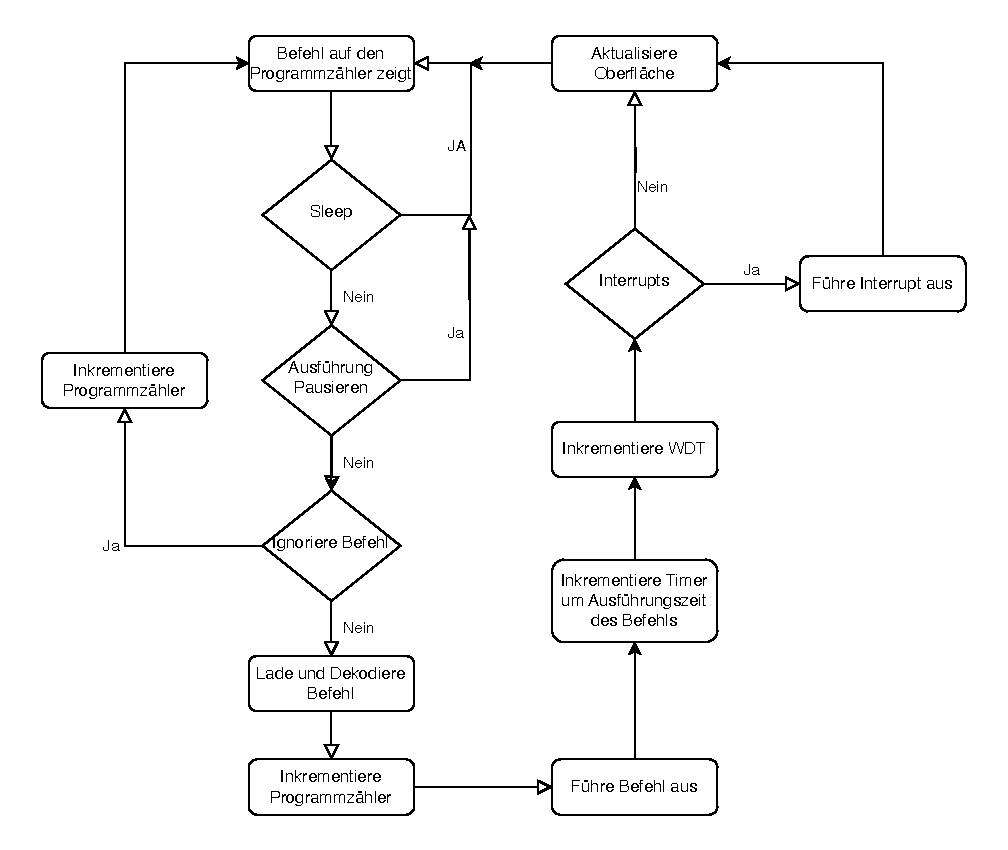
\includegraphics[width=\textwidth]{./img/excec_cycle.drawio.pdf}
    \caption{Programmablauf einer Befehlsausführung}
    \label{fig:execTask}
\end{figure}

\section{Detailierte Funktionsweise}
In diesem Abschnitt soll die genauere Funktionsweise verschiender Funktionen des Simulators anhand von einzelnen Beispielen erläutert werden. Dabei wird auf die einzelnen Module eingegangen und deren Funktionsweise erklärt.

% subwf
\subsection{subwf}
Der Befehl \texttt{subwf f,d} (Subtract W from f) subtrahiert den Inhalt des W-Registers (Arbeitsregister) vom Inhalt des Registers \texttt{f}. Das Ergebnis dieser Subtraktion wird dann, abhängig vom Wert des Destination-Bits \texttt{d}, entweder zurück in das W-Register (wenn \texttt{d=0}) oder in das Register \texttt{f} (wenn \texttt{d=1}) geschrieben. Bei dieser Operation werden die Statusbits C (Carry), DC (Digit Carry) und Z (Zero) im STATUS-Register entsprechend dem Ergebnis der Subtraktion beeinflusst. Wichtig zu beachten ist, dass das Carry Flag bei der Subtraktion invertiert ist.

\begin{lstlisting}[caption={Methode subwf aus dem \ac{ALU} Modul}, label={lst:subwf}]
def subwf(self, dest, reg_num):
    value = self.memory.readRegister(reg_num)
    result = value - self.memory.getW()
    self.memory.setBit(0x03, 0, 0 if result < 0 else 1)
    if result < 0:
        result = (result * (-1)-1) ^ 0xFF
    self.memory.setBit(0x03, 1, 0 if (value & 0x0F) - (self.memory.getW() & 0x0F) < 0  else 1)
    result = int(int(bin(result),2) & int('0b11111111',2))
    self.memory.setBit(0x03, 2, 1 if result == 0 else 0)

    self.memory.writeRegister(reg_num if dest else 'w', result)
\end{lstlisting}
\textbf{Erläuterung des Codes:}
Die Methode \texttt{subwf} (siehe Listing \ref{lst:subwf}) simuliert den gleichnamigen PIC-Befehl:
\begin{itemize}
    \item Zeile 2: Liest den Wert des Registers \texttt{f} (Operand \texttt{reg\_num}).
    \item Zeile 3: Subtrahiert den Inhalt des W-Registers vom gelesenen Wert \texttt{value}.
    \item Zeile 4: Setzt das Carry-Flag (C). Die Logik prüft, ob das \texttt{result} negativ ist. 
    \item Zeile 5-6: Ist das Ergebnis \texttt{result} negativ, wird es in das 8-Bit-Zweierkomplement umgewandelt (z.B. -1 zu 255).
    \item Zeile 7: Setzt das Digit-Carry-Flag (DC) korrekt, basierend auf einem Borrow bei der Subtraktion der unteren 4 Bits.
    \item Zeile 8: Maskiert \texttt{result} auf 8 Bit, um das Verhalten eines 8-Bit-Registers sicherzustellen.
    \item Zeile 9: Setzt das Zero-Flag (Z), falls das 8-Bit-\texttt{result} Null ist.
    \item Zeile 11: Schreibt das 8-Bit-\texttt{result} in das Zielregister: Register \texttt{f} (wenn \texttt{dest=1}) oder W-Register (wenn \texttt{dest=0}).
\end{itemize}

% call
\subsection{call}
Der Befehl \texttt{call k} (Call Subroutine) ruft ein Unterprogramm auf, das sich an der Adresse \texttt{k} befindet. Bevor der Sprung zur Adresse \texttt{k} ausgeführt wird, wird die Adresse des nächsten Befehls (der aktuelle Programmzähler + 1) auf dem Stack gespeichert. Dies ermöglicht die Rückkehr aus dem Unterprogramm mit einem \texttt{return}, \texttt{retlw} oder \texttt{retfie} Befehl. Die Zieladresse \texttt{k} ist eine 11-Bit-Adresse. Die oberen Bits des 13-Bit-Programmzählers werden aus dem PCLATH-Register geladen.

\begin{lstlisting}[language=Python, caption={Ausschnitt der CALL-Befehlsimplementierung im \acl{CPU} Modul}, label={lst:call}]
case 'call':
    self.stack.push(self.dMemory.getPCounter())
    pclath = int(("".join([str(x) for x in self.dMemory.memory[1][0x0A]])[3:5]),2) << 3
    val = bin(inst[1])[2:]
    pc = (pclath << 8) + int(val,2)
    self.dMemory.setPCounter(pc)
    self.dMemory.setPCL(self.dMemory.getPCounter() & 0xFF)
    self.addClockCycle()
\end{lstlisting}

\textbf{Erläuterung des Codes:}
Die Methode simuliert die Ausführung des \texttt{call}-Befehls (siehe Listing \ref{lst:call}):
\begin{itemize}
    \item Zeile 2: Die aktuelle Adresse des Programmzählers (\texttt{self.dMemory.getPCounter()}), welche auf den Befehl nach dem \texttt{call} zeigt, wird auf den Stack gelegt. Dies ist die Rücksprungadresse.
    \item Zeile 3: Die Bits 4 und 3 des PCLATH-Registers (Register an Adresse 0x0A, hier in Bank 1 angenommen) werden ausgelesen, zu einem Integer konvertiert und um 3 Bits nach links verschoben. Diese bilden einen Teil der oberen Bits der Zieladresse. Die komplexe String-Konstruktion dient dazu, die Bitwerte aus der Speicherrepräsentation zu extrahieren.
    \item Zeile 4: Der 11-Bit-Operandenwert \texttt{k} des \texttt{call}-Befehls (gespeichert in \texttt{inst[1]}) wird in seine binäre Stringrepräsentation ohne das Präfix \texttt{0b} umgewandelt.
    \item Zeile 5: Die vollständige 13-Bit-Zieladresse (\texttt{pc}) wird zusammengesetzt. Der in Zeile 3 berechnete Wert aus PCLATH wird um weitere 8 Bits nach links verschoben (insgesamt also um 11 Bits) und mit dem 11-Bit-Wert \texttt{val} (konvertiert zu Integer) addiert (bzw. OR-verknüpft, da \texttt{val} die unteren 11 Bits darstellt).
    \item Zeile 6: Der Programmzähler wird auf die neu berechnete Zieladresse \texttt{pc} gesetzt.
    \item Zeile 7: Das PCL-Register (Program Counter Low Byte, typischerweise Teil des Datenspeichers und Spiegel des PC<7:0>) wird mit den unteren 8 Bits des neuen Programmzählers aktualisiert.
    \item Zeile 8: Die Anzahl der Taktzyklen wird erhöht, da ein \texttt{call}-Befehl üblicherweise zwei Taktzyklen benötigt.
\end{itemize}

% decode \subsection{decode}
Die \texttt{decode}-Methode ist ein zentraler Bestandteil des Simulators und dafür zuständig, einen 14-Bit Maschinenbefehl (Opcode), der als Hexadezimalwert \texttt{cmd} übergeben wird, zu analysieren und in eine für die \ac{CPU} verständliche Struktur zu übersetzen. Diese Struktur besteht typischerweise aus dem Namen des Befehls (z.B. "bcf"), dem ersten Operanden (oft eine Registeradresse oder ein Literalwert) und dem zweiten Operanden (oft ein Bit-Index oder das Ziel-Bit).

\begin{lstlisting}[language=Python, caption={Ausschnitt der Decode-Methode im Decode-Modul}, label={lst:decode}, basicstyle=\ttfamily\footnotesize, numbers=left, numberstyle=\tiny\color{gray}]
# Opcode-Format: xxxx xxbb bfff ffff (b=Bit, f=Register)
# Beispiel: bcf f,b -> Opcode 01 00bb bfff ffff
# self.mask2 = 0x3C00 (11 1100 0000 0000) -> Isoliert die Bits 13-10
# self.fmask = 0x007F (00 0000 0111 1111) -> Isoliert die unteren 7 Bits (Register f)

    # cmd ist der 14-Bit Opcode als Integer
    masked2 = cmd & self.mask2 # Maskiert den Opcode, um die Befehlsgruppe zu identifizieren
    match masked2:
        #bcf (Bit Clear f) -> Opcode-Gruppe 0100 xxxx xxxx xxxx
        case 0x1000: # 0x1000 entspricht 0100 0000 0000 0000 (maskiert)
            return ("bcf", cmd & self.fmask, self.getBit(cmd))
        #bsf (Bit Set f) -> Opcode-Gruppe 0101 xxxx xxxx xxxx
        case 0x1400: # 0x1400 entspricht 0101 0000 0000 0000 (maskiert)
            return ("bsf", cmd & self.fmask, self.getBit(cmd))
        #btfsc (Bit Test f, Skip if Clear) -> Opcode-Gruppe 0110 xxxx xxxx xxxx
        case 0x1800: # 0x1800 entspricht 0110 0000 0000 0000 (maskiert)
            return ("btfsc", cmd & self.fmask, self.getBit(cmd))
        #btfss (Bit Test f, Skip if Set) -> Opcode-Gruppe 0111 xxxx xxxx xxxx
        case 0x1C00: # 0x1C00 entspricht 0111 0000 0000 0000 (maskiert)
            return ("btfss", cmd & self.fmask, self.getBit(cmd))
        #movlw (Move Literal to W) -> Opcode-Gruppe 1100 xxxx xxxx xxxx
        case 0x3000: # 0x3000 entspricht 1100 0000 0000 0000 (maskiert)
            return ("movlw", cmd & self.mask8, None) # self.mask8 = 0x00FF
        #retlw (Return with Literal in W) -> Opcode-Gruppe 1101 xxxx xxxx xxxx
        case 0x3400: # 0x3400 entspricht 1101 0000 0000 0000 (maskiert)
            return ("retlw", cmd & self.mask8, None) # self.mask8 = 0x00FF
        case _:
            pass 
\end{lstlisting}

\textbf{Erläuterung des Codes:}
Das Prinzip der \texttt{decode}-Methode (siehe Listing \ref{lst:decode}) beruht darauf, den übergebenen Maschinenbefehl \texttt{cmd} schrittweise zu analysieren, um die spezifische Operation und deren Operanden zu identifizieren.
\begin{itemize}
    \item Zeile 5: Der Opcode \texttt{cmd} wird mit einer Bitmaske (\texttt{self.mask2}, hier z.B. \texttt{0x3C00} bzw. \texttt{11110000000000}) bitweise UND-verknüpft. Diese Maske ist so gewählt, dass sie einen bestimmten Teil des Opcodes isoliert, der für eine Gruppe von Befehlen charakteristisch ist. Das Ergebnis \texttt{masked2} repräsentiert diese Befehlsgruppe.
    \item Zeile 6-23: Eine \texttt{match-case}-Struktur vergleicht \texttt{masked2} mit vordefinierten Werten, die den einzelnen Befehlsgruppen entsprechen.
    \item Zeile 8 (Beispiel \texttt{bcf}): Trifft der \texttt{case 0x1000} zu (was bedeutet, dass die oberen relevanten Bits des Opcodes dem Muster für \texttt{bcf} entsprechen), wird ein Tupel zurückgegeben.
    \begin{itemize}
        \item Das erste Element ist der Name des Befehls als String: \texttt{"bcf"}.
        \item Das zweite Element ist der erste Operand. Für \texttt{bcf f,b} ist dies die Registeradresse \texttt{f}. Sie wird extrahiert, indem \texttt{cmd} mit einer weiteren Maske (\texttt{self.fmask}, z.B. \texttt{0x007F}) verknüpft wird, die nur die Bits für die Registeradresse isoliert.
        \item Das dritte Element ist der zweite Operand, hier der Bitindex \texttt{b}. Dieser wird durch die Methode \texttt{self.getBit(cmd)} extrahiert, welche die entsprechenden Bits aus \texttt{cmd} isoliert und als Integer zurückgibt.
    \end{itemize}
    \item Zeilen 11-20: Analog werden andere Befehle wie \texttt{bsf}, \texttt{btfsc}, \texttt{btfss}, \texttt{movlw} und \texttt{retlw} dekodiert. Bei \texttt{movlw k} beispielsweise wird das 8-Bit-Literal \texttt{k} mit \texttt{cmd \& self.mask8} extrahiert, und der dritte Operand ist \texttt{None}, da dieser Befehl nur einen Operanden hat.
    \item Zeile 22: Wenn keine der vorherigen Bedingungen zutrifft, wird \texttt{pass} ausgeführt, was bedeutet, dass der Code zu weiteren \texttt{match-case}-Blöcken oder einer Fehlerbehandlung übergehen würde (nicht im Ausschnitt gezeigt).
\end{itemize}
Diese Methode ist notwendig, damit der Simulator die rohen, numerischen Befehlscodes, die aus der LST-Datei oder dem Programmspeicher gelesen werden, in eine Form umwandeln kann, mit der die \ac{CPU} Logik arbeiten kann, um die entsprechenden Aktionen (wie Registermanipulationen, Speicherzugriffe oder Sprünge) auszuführen.

% read register

\subsection{readRegister}

Die Methode \texttt{readRegister} ist eine Funktion des Speichermoduls, die den Inhalt eines bestimmten Registers im Datenspeicher des simulierten Mikrocontrollers liest. Diese Methode ist entscheidend für die Interaktion zwischen der \ac{CPU} und dem Speicher, da sie es der \ac{CPU} ermöglicht, auf die Werte in den Registern zuzugreifen, die für die Ausführung von Befehlen benötigt werden.

\begin{lstlisting}[language=Python, caption={Ausschnitt der readRegister-Methode im Speichermodul}, label={lst:readRegister}]
def readRegister(self, register: int, bank=None) -> int:
    if register == 'w':
        return self.WREG
    elif register in range(0x00, 0x80):
        if register == 0:
            register = self.readRegister(4)
        bank = self.getActiveBank() if bank == None else bank
        return int(("".join([str(x) for x in self.memory[bank][register]])),2)
    else:
        raise ValueError("Invalid register address")
\end{lstlisting}
\textbf{Erläuterung des Codes:}
Die Methode \texttt{readRegister} (siehe Listing \ref{lst:readRegister}) dient zum Auslesen von Werten aus den Registern des simulierten PIC-Mikrocontrollers.
\begin{itemize}
    \item Zeile 2-3: Wenn als \texttt{register} der String \texttt{'w'} übergeben wird, gibt die Methode direkt den Inhalt des W-Registers (\texttt{self.WREG}) zurück.
    \item Zeile 4: Prüft, ob die angeforderte Registeradresse im gültigen Bereich einer Speicherbank liegt (hier \texttt{0x00} bis \texttt{0x7F}).
    \item Zeile 5-7: Behandelt den Sonderfall der indirekten Adressierung. Wenn Register 0 (INDF - Indirect File) gelesen werden soll, wird stattdessen der Inhalt des FSR-Registers (File Select Register, Adresse 0x04) als die eigentliche Zieladresse interpretiert. Die Methode ruft sich also rekursiv mit der Adresse des FSR auf, um dessen Inhalt zu erhalten, welcher dann als neue \texttt{register}-Adresse verwendet wird.
    \item Zeile 9: Bestimmt die zu verwendende Speicherbank. Wenn der optionale Parameter \texttt{bank} nicht explizit übergeben wurde (\texttt{None}), wird die aktuell aktive Bank über \texttt{self.getActiveBank()} ermittelt. Andernfalls wird die übergebene \texttt{bank} verwendet.
    \item Zeile 13: Greift auf den Speicher zu. \texttt{self.memory[current\_bank][register]} adressiert das spezifische Register in der gewählten Bank. Wichtig ist hierbei, dass jedes Register als ein Array von 8 Elementen (Bits, z.B. \texttt{[0,1,0,1,0,1,0,1]}) gespeichert ist. Dieser Array wird zuerst in einen String aus Nullen und Einsen umgewandelt (z.B. \texttt{"01010101"}) und dann mittels \texttt{int(..., 2)} als Binärzahl interpretiert und in einen Integer-Wert konvertiert.
    \item Zeile 16-17: Wenn die angegebene Registeradresse ungültig ist (außerhalb des erwarteten Bereichs und nicht 'w'), wird ein \texttt{ValueError} ausgelöst.
\end{itemize}
Diese Funktion ist fundamental, da viele PIC-Befehle Registerinhalte lesen müssen, um Operationen auszuführen oder Entscheidungen zu treffen. Die korrekte Bankauswahl ist dabei entscheidend für die Korrektheit der Simulation.
\chapter{Fazit}

Nach Abschluss des PIC Simulator-Projekts können wir mit Stolz festhalten, dass alle ursprünglich definierten Anforderungen erfolgreich umgesetzt wurden. 

Der entwickelte Simulator bietet eine umfassende und benutzerfreundliche Lösung zur Simulation von PIC-Mikrocontroller-Programmen und stellt damit eine wertvolle Alternative zur physischen Hardware dar. Folglich konnten die zu Beginn des Projekts definierten Ziele entsprechend umgesetzt werden. Der PIC Simulator ermöglicht es Entwicklern Programme zu testen und zu debuggen, ohne auf physische Hardware angewiesen zu sein.

Zudem konnte durch das Projekt, dass Wissen über den PIC Mikrocontroller und die zugrunde liegende Architektur vertieft werden. Dies ist besonders wertvoll für zukünftige Projekte, in denen PIC-Mikrocontroller eingesetzt werden sollen.

\section{Herausforderungen im Entwicklungsprozess}

Trotz des erfolgreichen Abschlusses des Projekts gab es während der Entwicklung einige Herausforderungen:

\subsection{Integration von UI und Backend}

Eine der größten Herausforderungen war die nahtlose Integration der Benutzeroberfläche mit dem Backend. Die konstante Kommunikation zwischen diesen beiden Komponenten erwies sich als komplexer als zunächst angenommen:

\begin{itemize}
    \item \textbf{Asynchrone Aktualisierungen}: Die Notwendigkeit, die UI in Echtzeit zu aktualisieren, während das Backend die Simulation durchführt, erforderte eine sorgfältige Implementierung von asynchronen Mechanismen.
    \item \textbf{Datenfluss}: Die effiziente Übertragung von Daten zwischen Backend und Frontend musste optimiert werden, um nicht unnötig Ressourcen zu verbrauchen.
    \item \textbf{Ereignisbehandlung}: Die Verarbeitung von Benutzereingaben und deren korrekte Weiterleitung an die enstprechenden Backend Komponenten erfordete eine detailierte Einarbeitung in das Signal-Slot-System von Qt.
\end{itemize}

Die Lösung dieser Herausforderungen wurde durch den Einsatz von Python und Qt erreicht, die ein robustes Signal-Slot-System für die Kommunikation zwischen den Komponenten bereitstellen.

\subsection{Kontinuierliche Weiterentwicklung}

Ein weiterer anspruchsvoller Aspekt war die kontinuierliche Weiterentwicklung des Projekts. Während der Implementierung entstanden immer wieder neue Anforderungen und Herausforderungen:

\begin{itemize}
    \item \textbf{Erweiterung der Funktionalität}: Mit fortschreitender Entwicklung wurden zusätzliche Funktionen identifiziert, die integriert werden mussten, ohne die bestehende Codebasis zu beeinträchtigen. Teilweise mussten bestehende Module umgeschrieben werden, um neue Funktionalitäten zu unterstützen.
    \item \textbf{Fehlerbehandlung}: Mit zunehmender Komplexität des Systems musste ein robustes Fehlerbehandlungssystem entwickelt werden, um mit unerwarteten Situationen umgehen zu können.
\end{itemize}

Der modulare Aufbau des Simulators erwies sich hier als entscheidender Vorteil, da er die schrittweise Erweiterung und Anpassung des Systems ermöglichte, ohne die Gesamtstabilität zu gefährden.

\section{Lessons Learned}

Aus diesem Projekt haben wir wertvolle Erkenntnisse gewonnen:

\begin{itemize}
    \item \textbf{Vorausschauende Planung}: Eine gründliche Anforderungsanalyse und architektonische Planung zu Beginn des Projekts zahlen sich in späteren Phasen aus.
    \item \textbf{Modularität}: Ein modularer Ansatz ermöglicht flexiblere Anpassungen und Erweiterungen während der Entwicklung. 
    \item \textbf{Dokumentation}: Eine umfassende Dokumentation erleichtert die Wartung und Weiterentwicklung des Systems.
\end{itemize}




\appendix
\addcontentsline{toc}{chapter}{Anhang}

\addcontentsline{toc}{chapter}{Index}
\printindex


\end{document}
